
\subsection{Ruby on Rails}
\label{sec:rails}

Für das Projekt IT-jobs-und-stellen.de soll das Webframework Ruby-on-Rails verwendet werden. Rails wurde 2006 von der Firma 37signals unter der Leitung von David Heinemeier Hansson entwickelt und erlangte seitdem eine wachsende Popularität. Rails inspirierte viele andere Frameworks, wie z.B. cakePHP, Groovy on Grails, Symfony und ASP.NET MVC.

\marginline{
\includegraphics[width=0.8\marginparwidth]{material/rails.png}}
Viele professionelle Websites, die meist als Startup begannen, setzen bis heute auf Rails. Darunter z.B. Yellow Pages, die Gelben Seiten der USA, Github, eine sehr beliebte Community für OpenSource Programmierer,  Groupon, dem führenden Unternehmen bei Online-Gutscheinen und XING, einer deutschen Online-Community für Business-Kontakte.
% TODO http://rubyonrails.org/applications

%TODO Quelle http://www.businessinsider.com/heres-why-ruby-on-rails-is-hot-2011-5
Im Folgenden werden die Grundzüge von Ruby on Rails näher erläutert.

\subsubsection{Konzepte von Rails}
\label{sec:railsconcepts}
Rails ist ein Webframwork, das auf dem Model-View-Controller-Pattern basiert, welches eine 3-schichten Architektur darstellt. Jede Schicht hat fest definierte Aufgaben. Diese bilden normalerweise ein Dreigespann, bei Rails "`Ressource"` gennannt. Im folgenden werden die Schichten kurz erläutert, und am Beispiel einer Ressource "'Job"` 
\begin{description}
 \item[Model] In Klassen dieser Schicht werden Zugriffe auf die Persistenzschicht vorgenommen. Meist geschieht dies durch Ausführung von SQL-Befehlen auf eine relationale Datenbank. Innerhalb von Rails ist dies aber meist nicht notwendig, da das ORM\footnote{Objektrelationale Framework} ActiveRecord häufig verwendete SQL-Befehle abstrahiert. Auch die Geschäftslogik soll per Definition zu großem Teil in dieser Schicht erfolgen.
 
 Für einen Job ist das ein Modell, welches die Datenbanktabelle "'jobs"` anspricht, und z.B. die Attribute "'titel"`, "'datum"` und "'beschreibung"` besitzt. Dabei können auf diesem Level auch datenbankunabhängige Constraints definiert werden, z.B. dass ein Job nur dann gespeichert werden soll, wenn der Titel mindestens 20 Zeichen lang ist, und das Datum mindestens das heutige ist.
 \item[Controller] Klassen dieser Schicht vereinigen Methoden, die von außen per HTTP erreichbar sind. Diese Methoden kommunizieren mit den korrespondierenden Models und bestimmen, welche View im einzelnen ausgeliefert wird. Weitere Funktionen eines Controllers sind Authentifizierung und Autorisierung (Wer darf was).\\
 Standardmäßig stellt Rails die CRUD\footnote{Create Read Update Delete}-Operationen bereit, welche in Form eines REST\footnote{Representational State Transfer die HTTP-Methoden GET, POST, PUT, DELETE werden in Kombination mit einem definierten URL-Schema direkt auf die Aktionen \texttt{Auflisten, Anzeigen, Bearbeiten, Löschen, Neu anlegen} gemappt.
 \url{http://en.wikipedia.org/wiki/Representational_State_Transfer}}
 \item[View] Eine View ist in der Regel ein Stück HTML Code welches einem Model zugeordnet ist, das bei einer bestimmten Aktion dem Clienten ausgeliefert wird. Neben HTML ist auch Javascript oder XML eine mögliche Auslieferungsform.\\
 Für den Job wäre das eine View für die Liste aller Jobs, einen Job im Detail anzeigen sowie das Formular zum Anlegen und Bearbeiten eines Jobs.
 \end{description}
 \begin{figure}[h]
  \centering
  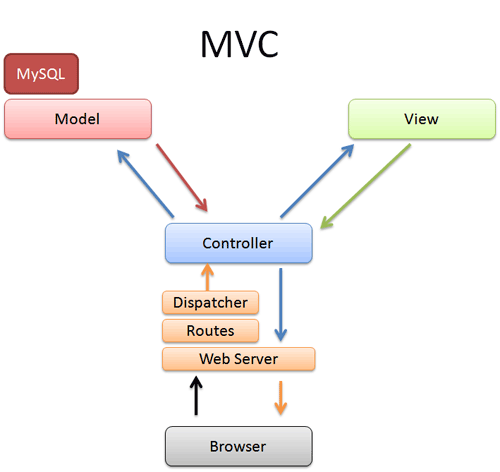
\includegraphics[width=0.7\textwidth]{./material/mvc-rails.png}
  % mvc-rails.png: 500x472 pixel, 72dpi, 17.64x16.65 cm, bb=
  % SOURCE  
  \caption{MVC Modell von Rails}
  \caption*{Quelle: \href{http://betterexplained.com/articles/intermediate-rails-understanding-models-views-and-controllers/}{betterexplained.com}}
 \label{fig:mvcrails}
\end{figure}
In Abbildung \ref{fig:mvcrails} ist der Ablauf einer Anfrage an den Server dargestellt. Die Anfrage des Browsers an die Website \texttt{http://localhost/jobs/12} wird über den Webserver, z.B. Apache2, an die Railsanwendung gestellt. Innerhalb von Rails wird dieser Anforderungsstring anhand der Routen, die die Anwendung anbietet, gematcht. In unserem Falle würde \texttt{/jobs/12} auf den Controller jobs aufgelöst werden. Innerhalb dieses Controllers wird eine Methode (Aktion) show erwartet.
Diese Methode wird nun ihrerseits eine Anfrage an das Model Job stellen, den Job mit der ID 12 aus der Datenbank zu holen. Danach wird ein HTML Template zur Detailanzeige des Jobs generiert.

\setlength{\epigraphwidth}{\marginparwidth}
\marginline{\epigraph{Ruby on Rails is a breakthrough in lowering the barriers of entry to programming. Powerful web applications that formerly might have taken weeks or months to develop can be produced in a matter of days.}{Tim O'Reilly, Founder of O'Reilly Media}}
\setlength{\epigraphwidth}{0.8\textwidth}

Neben diesem architektorischen Konzept verfolgt Rails noch andere Strategien, um das Entwickeln produktiver zu gestalten.
\begin{description}
 \item[Convention over Configuration] Rails ist so konzipiert, um als Framework komplett out-of-the-box zu funktionieren. Außer die Datenbankeinstellung wird keine Konfiguration im Vorderfeld benötigt. Diese Methodology zieht sich auch durch das Ökosystem durch. Die meisten externen Bibliotheken, bei Ruby Gems genannt, funktionieren bereits nach wenigen Kommandos. Dies macht das prototypische Entwickeln äußert effektiv. Weiterhin ist die Struktur eines Railsprojektes extrem fest definiert. So gibt es u.a. einen Ordner "'app"` mit den Model, Controller und View Dateien und einen Ordner "'test"`, der wiederrum in "'unit"`, "'functional"`, "'integration"` und "'performance"` unterteilt ist. So finden sich Railsprogrammierer auch in fremden Projekten sofort zurecht.
 \item[Don't repeat yourself (DRY)] Hier ist das Ziel, die Duplikation soweit wie möglich zu reduzieren, und das ständige Auslagern und Refaktorisieren des Codes, um bei Änderungen nur an einer Stelle ansetzen zu müssen. Ein weiteres Beispiel ist die Definition der Spalten des ORMs. Im Gegensatz zu anderen ORM-Frameworks ist diese bei Rails nicht notwendig. Rails erstellt automatisch Getter und Setter für die in der Datenbank definierten Tabellenspalten.
 \item[REST] Representational State Transfer ist Software-Architektur für HTTP-WebServices. Dabei werden neben den Standard HTTP Methoden GET und POST auch die selten benutzen Verben DELETE und PUT verwendet, um Aktionen auf einer Ressource zu definieren. Das Ziel ist ein sehr einfaches Design der URLs. Hier folgt die Auflistung der vier CRUD Operationen plus Auflistenvon REST am Beispiel einer Ressource "'jobs"` eines Webservice
 \begin{description}
  \item[GET /jobs.html] Auflisten aller Jobs, Ausgabe als HTML Format
  \item[GET /jobs/12.xml] Job mit der ID 12 anzeigen, Formatiere als XML
  \item[POST /jobs] Einen Job anlegen. Alle benötigten Parameter, wie Titel, Beschreibung oder Datum sollten im POST-Body der HTTP-Anfrage enthalten sein
  \item[PUT /jobs/12] Den Job mit der ID 12 aktualisieren. Die Eigenschaften, die aktualisiert werden, müssen wiederrum als Parameter mit übergeben werden
  \item[DELETE /jobs/12] Lösche den Job mit der ID 12
  \end{description} 
 Rails macht das Arbeiten im Kontext dieser Architektur sehr einfach, und es gilt als die bevorzugte Methode in der Community, APIs zu bauen. 
 \item[Codegeneratoren] Rails bietet viele Codegeneratoren an, um schnell benötigte Klassen und Datenbanktabellen anzulegen. Im Railsprojekt reicht z.B.:
\begin{lstlisting}
rails generate scaffold job title:string description:text \
  start_date:datetime active:boolean user:references
\end{lstlisting}
  Damit wird das Model Job, eine Erstellung der Tabelle "'jobs"`, ein Controller "'jobs"` mit den REST-Standardaktionen und entsprechenden Beispielviews, sowie Testfälle für Unit- und Funktionale Tests angelegt. Weiterhin sei zu bemerken, dass durch die Anweisung \texttt{user\:references} eine Spalte \texttt{user\_id} angelegt wird und eine 1:n-Beziehung zum Modell "'user"` hergestellt wird.
 \item[Full-Stack Webframework] Rails bringt out-of-the-box alles mit, was zur Webentwicklung benötigt wird. Im Gegensatz zu anderen Webframeworks wurde für Datenbankanbindung, Templatesystem, Javascriptframework, Testframework und Webserver-API bereits eine Vorauswahl getroffen. Im aktuellen Rails 3.1 sind dies ActiveRecord, ERB, JQuery, sowie Test::Unit und Rack. Die meisten dieser Teil-Frameworks lassen sich zwar leicht austauschen, Rails selbst aber proklamiert "'opinionated"`, also rechthaberisch/eigensinnig, zu sein, und den Entwickler Standards vorzugeben \citep{david_heinemeier_hansson_railsconf_2011}.
 \epigraph{Rails will have strong defaults. They might change over time but Rails will remain opinionated.}{David Heinemeier Hansson, Begründer von Rails}
\end{description}

Eine Einführung und Programmierung in Rails soll nicht Bestandteil dieser Diplomarbeit werden. Für eine weitere Einarbeitung seien die folgende Quellen insbesondere empfohlen:
\begin{description}
 \item[Rails for Zombies] Dies ist ein moderner, interaktiver Onlinekurs. Greg Pollack und das Team von RailsEnvy verpackt die Lektionen in humorige interaktive Lernerfahrungen. Jeweils eingeleitet durch ein Video muss der Teilnehmer Aufgaben direkt im Sourcecode lösen. Mithilfe dieses Kurses gelang es mir, meinen Arbeitskollegen einen guten Überblick über Rails zu verschaffen. Die Teilnahme ist kostenlos.\\
 \url{http://railsforzombies.org/}
 \item[Agile Webdevelopment with Ruby on Rails] Das quasi-Standardwerk. Wird meist parallel mit einer neuen Rails-Version in einer neuen Auflage gedruckt, aktuell die Dritte \citep{ruby_agile_2009}.
 \item[Rails Guides] Die von Ruby-on-Rails herausgegebenen "'Rails Guides"` sind eine gut strukturierte, kostenlose Online-Dokumentation, die nahezu alle Aspekte von Rails beleuchten.\\
 \url{http://guides.rubyonrails.org/getting_started.html}
 \end{description}



\subsubsection{Diskussion}
Nach einem kurzen Überblick über Rails, sollen nun die Eigenschaften des Frameworks diskutiert werden, und welche Auswirkungen sich dadurch auf das Testen ergibt.
\paragraph{Vorteile}
%TODO  a lot

Dank der Modularität können als Persistenzgrundlage sowohl relationale Datenbank, wie MySQL, SQlite und Oracle, aber auch andere Formen, wie NoSQL-Datenbanken transparent verwendet werden. Dank einer einfach zu verstehenden Syntax, ist das Schreiben von SQL in 95\% der Fälle überflüssig und zudem auch sicherer. Hier ein Beispiel, wie das Anlegen und Auslesen einer Instanz "'Vertragsart"` erfolgt. Parallel dazu als Kommentar die SQL Kommandos, die ActiveRecord im Hintergrund ausführt.
\begin{lstlisting}
c = ContractType.new
c.name = "Vollzeit"
c.save
=> false
#  SQL (0.1ms)  BEGIN
#  SQL (0.3ms)  SELECT 1 FROM `contract_types` 
#     WHERE (`contract_types`.`name` = BINARY 'Vollzeit') LIMIT 1
#  SQL (0.1ms)  ROLLBACK
>> c.errors
=> {:name=>["Name bereits vorhanden. Der Name muss einmalig sein"]}
>> c.name = "Praktikum"
>> c.save
=> true
#  SQL (0.1ms)  BEGIN
#  SQL (0.4ms)  SELECT 1 FROM `contract_types` 
#     WHERE (`contract_types`.`name` = BINARY 'Praktikum') LIMIT 1
#  SQL (0.4ms)  describe `contract_types`
#  AREL (0.4ms)  INSERT INTO `contract_types` (`name`) VALUES ('Praktikum')
#  SQL (7.1ms)  COMMIT
\end{lstlisting}
Hierbei ist auch schön zusehen, wie in Rails standardmäßig Transaktionen verwendet werden. Auch sieht man, wie eine Validierung funktioniert. Für das Modell VertragsArt wurde eine Einmaligkeit des Attributs name vereinbart. Dies prüft Rails vor dem Speichern und bricht das Speichern ab, falls eine Prüfung fehlschlug.

Die Implementation dieser Prüfung ist denkbar einfach.
\begin{lstlisting}
class ContractType < ActiveRecord::Base
  validates :name, :uniqueness => true, :presence => true
  
  has_and_belongs_to_many :jobs
end
\end{lstlisting}
Wir vereinbaren so, dass das Attribut Name einmalig sein muss (uniqueness), und ausgefüllt sein muss (presence). Die andere Zeile mit has\_and\_belongs\_to\_many definiert eine n:m Beziehung mit dem Modell Job, d.h. ein Job hat mehrere Vertragsarten. Der Rest geschieht dann durch Metaprogrammierung.

Mit minimalem Code lassen sich so komplexe Probleme abbilden. Dies macht Rails zu dem hochproduktivem Framework, als das es entwickelt wurde.
\epigraph{I needed to be way more productive...}{David Heinemeier Hansson}
%TODO Quote

Rails bietet eine gute Ausgangsbasis um sichere Websoftware zu entwickeln. Das Verwenden eines Datenbankframeworks macht SQL-Injections unmöglich. 
Cross-Site-Scripting
Cross-Site-Request-Forgery und Session-Angriffe werden erschwert, da Session und Cookie Variablen standardmäßig verschlüsselt werden.
Durch die Verwendung des

% SQL Injection
% Tower of Babel

\paragraph{Nachteile}
Interaktion mit Legacy-Software ist nicht immer möglich. ActiveRecord reserviert ein paar Spaltennamen, wie \texttt{type} und  class. Eine Benennung der Spalten sollte der Ruby-Namenskonvention entsprechen, also nur Buchstaben Zahlen und Unterstriche enthalten. Ansonsten können die Spalten nur über Umwege angesprochen werden.

\paragraph{Performance} Oft wird angeführt, dass Ruby als Skriptsprache und Rails als darauf aufbauendes Framework eine schlechte Performance hat, und dadurch ungeeignet für große Webanwendungen ist.
%TODO QUelle, wer sagt das?

%TODO Benchmark, Diskussion zur Architektur

Anderseits gibt es Anzeichen dafür, dass eine clevere Architektur und Caching für skalierende Anwendung entscheidender ist, als die letztendliche Ausführungszeit.

Das dies möglich ist, zeigen z.B. Groupon, der führende Online-Coupon-Anbieter mit mehr als 50 Mio Abonnenten und 
%TODO http://www.socialshopping.com/Groupon/news/Groupon-hits-50m-Subscribers-Shopping-site-sensation-201101210398/
Twitter, die jeweils Rails verwenden.
%TODO Quelle Rails applications

\paragraph{Rails und Tests}
Rails bietet ausgezeichnete Vorraussetzungen zum Softwaretest. Dafür sprechen, dass...

\begin{itemize}
 \item benötigte Bibliotheken bereits mitgliefert werden. Dies umfasst einen Test-Runner, vorkonfigurierte Test-Datenbanken (auf Basis von SQLite) und das Testframework Minitest,
 \item die Verwendung stark erleichtert wird, da Rails beim Nutzen der Codegeneratoren analoge Testdateien gleich mitgeneriert,
 \item neben den mitgelieferten Tools das Rails Ökosystem eine Vielzahl von Testtools bereitstellt, u.a. Rspec (BDD\footnote{Behavior Driven Development, siehe Glossar}-Testframework), Rcov (Testabdeckung), diverse Mockbibliotheken (mocha, FlexMock, RR, Rspec Mocks), Tools zum Generieren und Bereitstellen von Testdaten (Fixtures, Factories, Faker) und Codemetriken (metric-fu)
 \item das Testen einen sehr hohen Stellenwert in der Ruby und Rails-Comumnity hat. Nahezu alle namhaften Ruby-Programmierer schreiben umfassende Tests \citep{devries_rails_2008}. Das Resultat ist, dass auch fast alle OpenSource Bibliotheken (Gems) bei Ruby eine "`solid suite of tests"' haben \citep{devries_rails_2008}. 
\end{itemize}

Dabei werden mehrere verschiedene Testarten unterstützt und definiert.
\begin{description}
 \item[Unittests] oder Modelltests (model test). Zielstellung: Hier wird die Logik einer Modelklasse untersucht\\
 Testziel: alle (komplexeren) Methoden die das Modell anbietet. Am Beispiel Job kann das die Aussage sein, wann ein Job gültig ist, d.h. welche Bedingungen für die einzelnen Attribute gelten sollen.\\
 Testart: Whitebox
 \item[Funktionale Tests] Untersuchungsgegenstand sind die Controller, also die Schnittstellen zum Nutzer. \\
 Testziel: Getestet wird meist der Arbeitsablauf innerhalb eines Controllers, also Weiterleitungen, Benachrichtigungen und welches Template gerendert wird.\\
 Testart: Whitebox
 Es können auch oberflächliche View-Tests unternommen werden, also die Aussage ob ein bestimmtes HTML-Element auf der Seite zu sehen ist.
 \item[Integrationstests] es wird ein Browser simuliert der von außen auf die Applikation zugreift
 Zielstellung: Testen komplexer Interaktionen zwischen verschiedenen Teilen der Software\\
 Beispiel: Ein User loggt sich ein und legt einen neuen Job an\\
 Testart: Graybox oder Blackbox
 \item[Performanz-Tests] Eine Testart, die alle Methoden aus Unittests und Funktionalen Tests beinhaltet\\
 Zielstellung: Herausfinden von Performanz-Flaschenhälsen in allen Ebenen. \\
 Beispiel: Es werden 1000 Jobs generiert und geprüft, ob die Anzeige schnell genug läuft\\
 Testart: Graybox
\end{description}
